\documentclass[10pt]{article}

\usepackage[T1]{fontenc}
\usepackage[utf8]{inputenc}
\usepackage[margin=0.82in]{geometry}
\usepackage{amsmath,amssymb}
\usepackage{booktabs}
\usepackage{graphicx}
\usepackage{microtype}
\usepackage{tabularx}
\usepackage{xcolor}
\usepackage{hyperref}

\definecolor{linkblue}{HTML}{1F4D78}
\hypersetup{
  colorlinks=true,
  linkcolor=linkblue,
  citecolor=linkblue,
  urlcolor=linkblue,
  pdftitle={From Quantum Telepathy to Operational Quantum Advantage},
  pdfauthor={Quantum Network Simulator R&D Project}
}
\graphicspath{{figures/}}
\setlength{\parindent}{0pt}
\setlength{\parskip}{5pt}
\newcommand{\pass}{\textsc{pass}}
\newcommand{\partialstatus}{\textsc{partial}}

\title{From Quantum Telepathy to Operational Quantum Advantage\\
\large A Reproducible Simulator Study of Latency-Constrained Coordination}
\author{Quantum Network Simulator R\&D Project}
\date{September 3, 2026}

\begin{document}
\maketitle

\begin{abstract}
We present a version-pinned research simulator that connects the idealized
latency-constrained trading game of Ding and Jiang to the operational
nonlocal-game criteria of Li \emph{et al.}  The implementation separates the
game, physical-error, finite-statistics, decision-latency, and entanglement
supply layers.  Classical optima for binary games are independently verified
by exhaustive enumeration of deterministic local strategies.  We recover the
canonical CHSH utilities $\omega_C=0.75$ and
$\omega_Q=(1+1/\sqrt{2})/2$, reproduce representative Ding--Jiang results,
and implement asymmetric utilities and correlated inputs.  For the
representative 50-km system, lower-level parameters yield an entanglement rate
of $7854.545\,\mathrm{s}^{-1}$ and a local decision latency of
$0.970\,\mu\mathrm{s}$.  A 256-seed event-driven simulation gives a mean rate
of $7863.867\,\mathrm{s}^{-1}$ with a 95\% confidence interval of
$[7826.764,7900.970]\,\mathrm{s}^{-1}$.  A staged HFT analysis demonstrates
that a positive theoretical gap can still fail because of rate, fidelity,
decision, or no-communication constraints.  All 12 final reproduction jobs
and 592 pre-existing tests pass.  Published plots without pointwise author
data and microscopic device models without sufficient pulse information
remain explicitly partial or information-limited rather than being promoted
to successful reproductions.
\end{abstract}

\section{Introduction}

Latency-constrained task completion (LCTC) provides an operational setting in
which separated agents must act before ordinary communication can coordinate
their decisions.  Ding and Jiang introduced this structure for high-frequency
trading (HFT) and showed that preshared entanglement can improve expected
utility in an idealized model \cite{dingjiang2025}.  Li \emph{et al.} extended
the setting to finite stationary windows, asymmetric utilities, imperfect
states and measurements, finite statistics, finite entanglement supply, and
local decision latency \cite{li2026}.

The central methodological point is that
\begin{equation}
  \Delta\omega > 0
\end{equation}
is necessary but not sufficient for an operational claim.  An experiment or
application must also preserve enough fidelity, collect enough statistically
informative rounds within the environment stationary window, supply heralded
entanglement at the required rate, and finish the local quantum decision
inside the allowed window.  This work implements those tests in a single
traceable software architecture while preserving Ding--Jiang regression
results.

We reproduce Ding and Jiang arXiv:2407.21723v3 and Li \emph{et al.}
arXiv:2604.07451v1.  The former pin matters because its v2 revision corrected
the HFT example and v3 corrected the quantum-memory calculation.  We do not
combine equations or parameters from different versions.

\section{Model and Validation Architecture}

\subsection{Generic nonlocal games}

For inputs $x,y$, outputs $a,b$, input distribution $P(x,y)$, utility
$u(a,b\mid x,y)$, and behavior $P(a,b\mid x,y)$, the expected utility is
\begin{equation}
  \omega = \sum_{x,y,a,b} P(x,y)u(a,b\mid x,y)P(a,b\mid x,y).
  \label{eq:utility}
\end{equation}
For the two-input, two-output games used here, all 16 deterministic local
strategies are enumerated.  Since shared randomness only forms their convex
hull, the largest deterministic value is the admissible no-communication
classical optimum.

For a normalized XOR game with correlator matrix $M$, we denote its classical
and quantum biases by $C_b(M)$ and $Q_b(M)$.  The corresponding win utilities
are
\begin{equation}
  \omega_C=\frac{1+C_b(M)}{2}, \qquad
  \omega_Q=\frac{1+Q_b(M)}{2}.
  \label{eq:xorutilities}
\end{equation}
At the uniform CHSH point \cite{chsh1969}, the implementation recovers
\begin{align}
  \omega_C &= \frac{3}{4}, &
  \omega_Q &= \frac{1+1/\sqrt{2}}{2}, &
  \Delta\omega &= \frac{\sqrt{2}-1}{4}.
  \label{eq:chsh}
\end{align}
The numerical gap is $0.10355339059327373$.  The production XOR path, direct
utility sum, and deterministic enumeration agree to at most
$2.22\times10^{-16}$ on the configured benchmark grids.

\subsection{Layered implementation}

The simulator uses six scientific layers: (i) generic games and behaviors,
(ii) XOR/CHSH values, (iii) the Ding--Jiang HFT model, (iv) generalized Li LCTC
games, (v) exact physical-error and finite-statistics models, and (vi) M0/M1/M2
network hardware.  Application, network, and device parameters remain in
separate configuration fields.  Paper values are stored as validation oracles
rather than reused as hidden model inputs.

The oracle hierarchy is analytical solution, independently written
calculation, published numerical value or table, author data, digitized plot,
and Monte Carlo cross-validation.  The production implementation is never its
own oracle.  NPA $Q1+AB$ bounds used for lossy games follow the convergent
semidefinite hierarchy introduced by Navascues, Pironio, and Acin
\cite{npa2007}.

\section{Ding--Jiang Reproduction}

\subsection{Ideal HFT utility}

The Ding--Jiang HFT model uses correlated local financial observations,
preshared resources, and no communication after observation.  Figure
\ref{fig:dingfig3} shows the reproduced 101-by-101 utility-gap grid and selected
cross-sections.  The maximum occurs at the CHSH point $p=0.5$, $\beta=0$ (or
the relabeled $\beta=1$ point) and equals $0.10355339059327373$.  The gap is
zero at $\beta=0.5$, and the numerical grid satisfies the expected $\beta$
relabeling symmetry.

\begin{figure}[htbp]
  \centering
  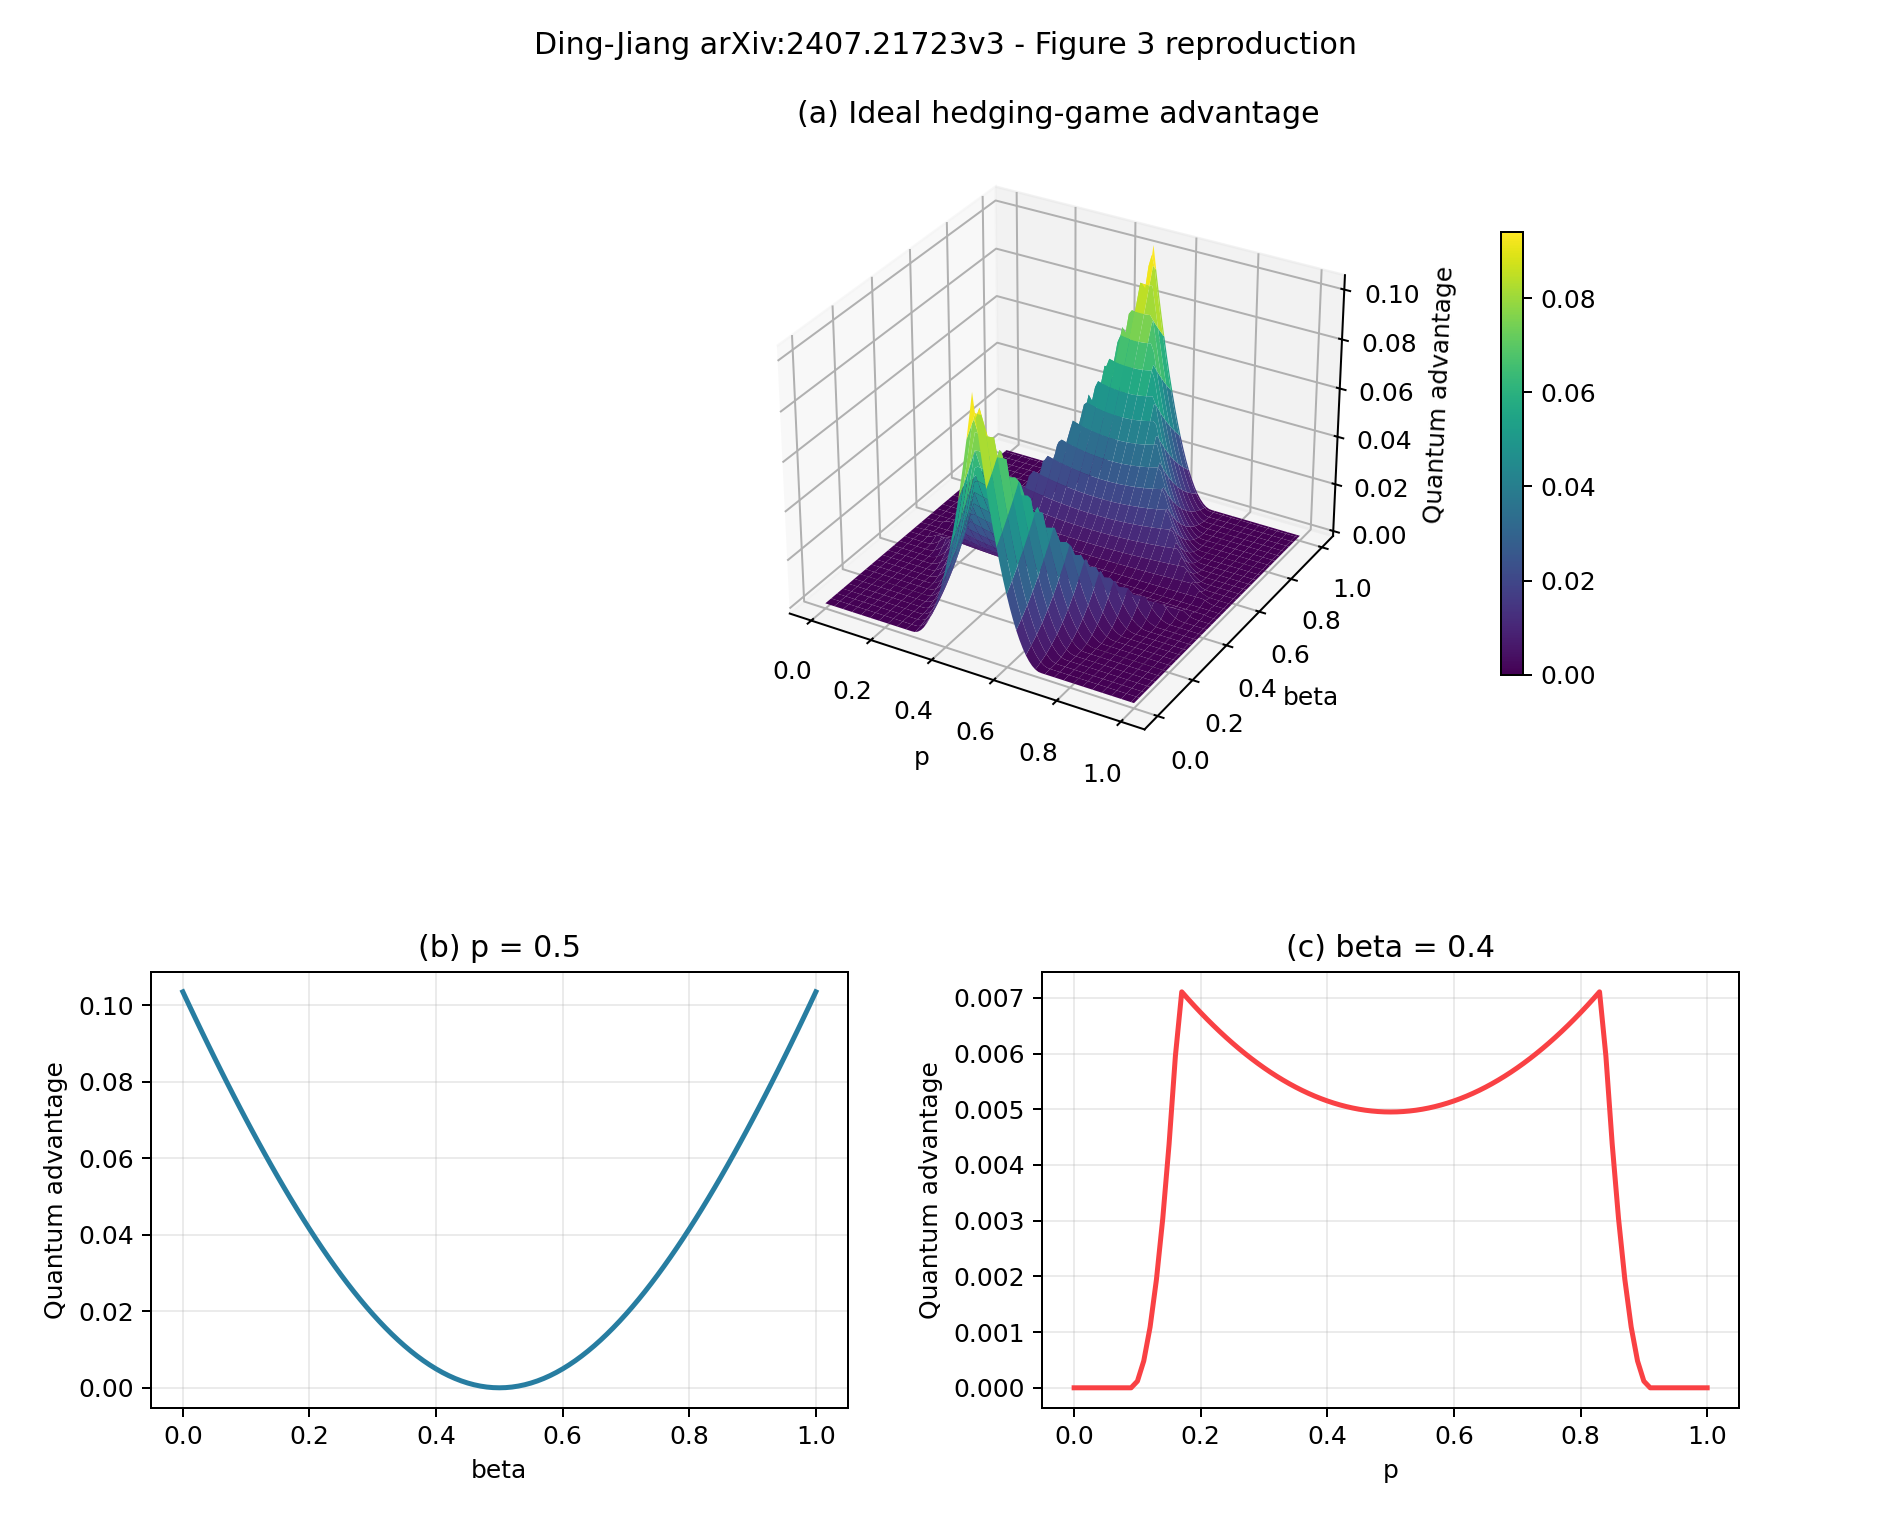
\includegraphics[width=0.92\linewidth]{ding_fig3.png}
  \caption{Equation-based reproduction of Ding--Jiang v3 Figure 3.  The
  maximum and symmetry checks are analytical validation gates.  Pointwise
  author grid data are unavailable, so the paper-level status remains
  \partialstatus.}
  \label{fig:dingfig3}
\end{figure}

For the representative lossy case $p=0.3$, $\beta=0.3$, the simulator obtains
the transition efficiency $\eta_\star=0.9405975342$, classical utility
$0.79$, and quantum utility $0.7918676876$.  The published rounded values are
$0.941$, $0.79$, and $0.792$.  Loss-threshold cross-sections use an explicit
two-qubit strategy as a lower bound and an independent $Q1+AB$ value as an
upper bound.  The full author surface and unpublished modified-NPA code are
not available; this target is therefore \partialstatus.

\subsection{Corrected v3 Type II memory calculation}

The corrected v3 two-arm transmission produces
\begin{equation}
  t_a=234.583333\,\mu\mathrm{s},\qquad
  p_s=0.0248360496,\qquad
  \frac{r_e}{M}=105.8730355\,\mathrm{Hz}.
\end{equation}
These values agree with the paper's rounded $230\,\mu\mathrm{s}$, $0.0248$,
and $106M\,\mathrm{Hz}$ statements.  One memory suffices for a target event
rate of $100\,\mathrm{Hz}$.  This M1 calculation intentionally excludes local
operation time, occupancy, reset, finite memory lifetime, and decoherence;
those effects enter separately in M2.

The Ding depolarizing model is implemented as an exact behavior mixture with
uniform binary outputs.  The maximum robustness threshold is
$0.2928932188134524$ at the CHSH point.  Figure-level checks against the
published robustness heatmaps are invariant- and equation-based because
author point grids are unavailable.

\section{Generalized LCTC and Physical Errors}

The Li model independently supports $\beta_1$, $\beta_2$, and arbitrary
correlated $P(x,y)$.  It reduces exactly to the Ding utility after the global
parity relabeling used in the paper.  The sign of the bottom-right game-matrix
entry follows the expanded utility and the uniform CHSH limit; a conflicting
displayed sign in Eq. 25 is recorded as a source discrepancy.

Figure \ref{fig:lifig2} reproduces the independent-input, correlated-input,
and noisy-gap panels.  The independent family reaches the CHSH gap
$0.1035533906$.  The configured correlated family reaches $0.0674234614$ at
$P(1,1)=0.4$ and $\beta_1=\beta_2=0$, with utilities $0.8$ and
$0.8674234614$.

\begin{figure}[htbp]
  \centering
  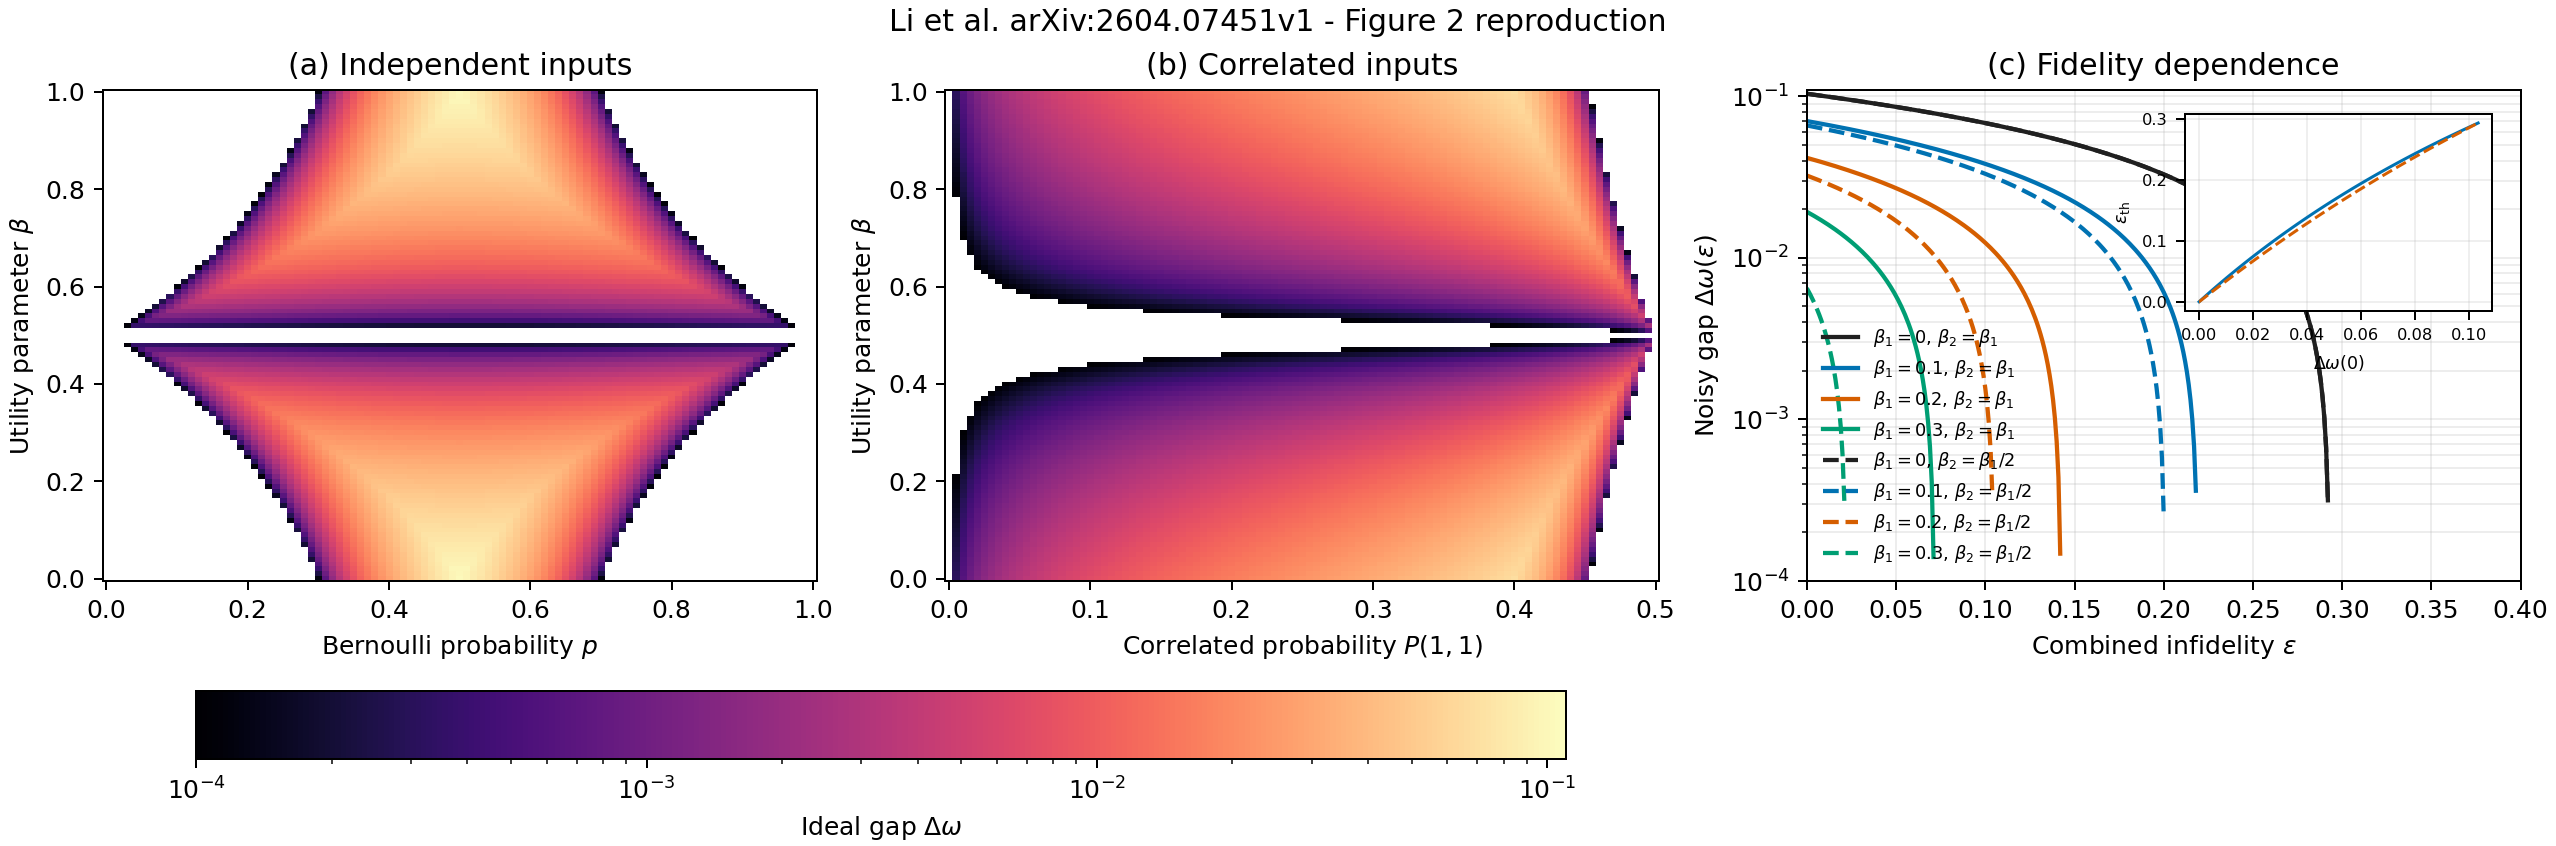
\includegraphics[width=0.96\linewidth]{li_fig2.png}
  \caption{Reproduction of Li \emph{et al.} Figure 2: ideal independent and
  correlated input families and exact combined-infidelity dependence.}
  \label{fig:lifig2}
\end{figure}

The state is a Werner mixture with state infidelity $\epsilon_s$ and each
binary measurement has outcome-flip infidelity $\epsilon_{\mathrm{meas}}$.
The exact combined infidelity is
\begin{equation}
  \epsilon = 1-\left(1-\frac{4\epsilon_s}{3}\right)
  (1-2\epsilon_{\mathrm{meas}})^2.
  \label{eq:combinederror}
\end{equation}
No small-error approximation is substituted for Eq. \eqref{eq:combinederror}.
For $\epsilon_s=0.04$ and $\epsilon_{\mathrm{meas}}=0.002$, it gives
$\epsilon=0.06089152$.

The fidelity condition is
\begin{equation}
  \epsilon < \epsilon_{\mathrm{th}}(M), \qquad
  \epsilon_{\mathrm{th}}(M)=1-\frac{C_b(M)}{Q_b(M)}.
  \label{eq:fidelity}
\end{equation}
For CHSH this becomes $1-1/\sqrt{2}=0.2928932188$.

\section{Finite Statistics and Operational Criteria}

For a binary win/loss game, let $w_n=\lceil n\omega_Q(\epsilon)\rceil$ be the
expected quantum win count rounded to the first certifying integer.  The
classical null-model $p$-value is evaluated with the stable exact upper tail
\begin{equation}
  p_n=\sum_{k=w_n}^{n}{n\choose k}
  \omega_C^k(1-\omega_C)^{n-k}.
  \label{eq:binomial}
\end{equation}
The required rounds are the smallest integer $n_{\mathrm{req}}$ satisfying
$p_n<\alpha$, and the required trial rate is
\begin{equation}
  R_{\mathrm{req}}=\frac{n_{\mathrm{req}}}{T_{\mathrm{env}}}.
  \label{eq:rreq}
\end{equation}
Small-$n$ results are independently checked using 60-digit Decimal direct
sums.  General bounded scores use the conservative Li Eq. 20 bound in log
space, with discrete minimality verified independently.

At $\epsilon=0.061$, $n_{\mathrm{req}}=65$ for $\alpha=0.05$ and
$n_{\mathrm{req}}=238$ for $\alpha=0.001$.  Figure \ref{fig:lifig3} shows that
$R_{\mathrm{req}}$ increases sharply as the fidelity threshold is approached.
For a $1\,\mathrm{ms}$ stationary window and $\alpha=0.05$, the required rate
is $65\,\mathrm{kHz}$ and a $7.9\,\mathrm{kHz}$ system fails.  For
$T_{\mathrm{env}}=100\,\mathrm{ms}$, the required rate is
$650\,\mathrm{s}^{-1}$ and the same system passes.

\begin{figure}[htbp]
  \centering
  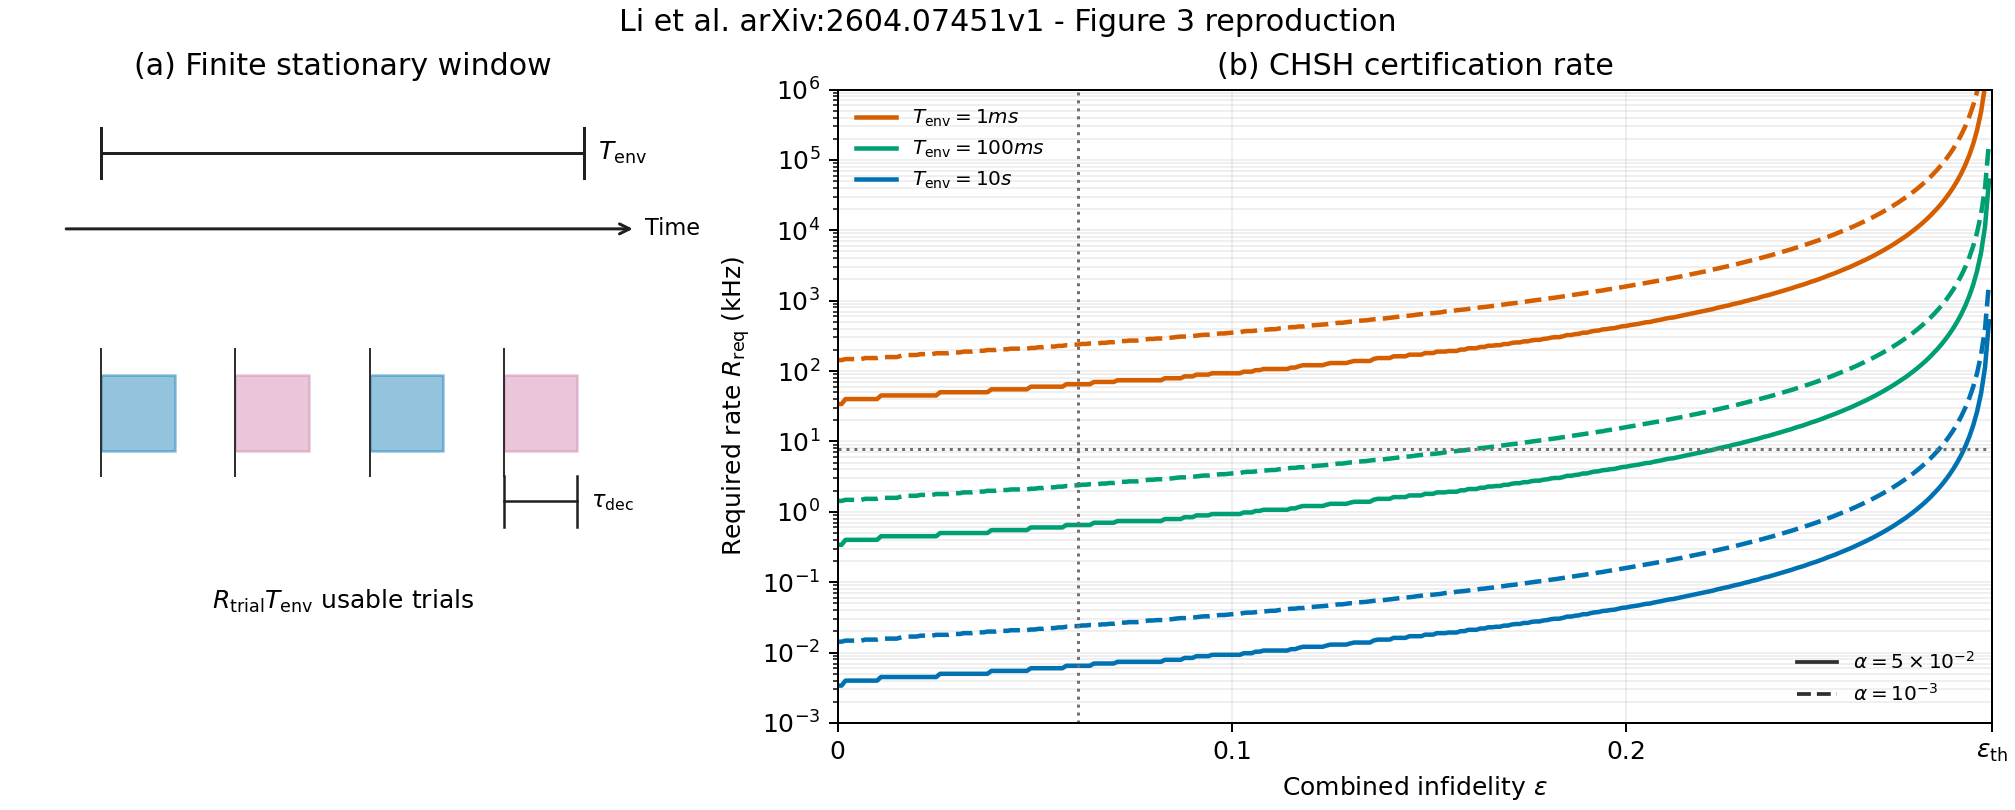
\includegraphics[width=0.94\linewidth]{li_fig3.png}
  \caption{Finite-statistics rate reproduction corresponding to Li
  \emph{et al.} Figure 3.  Curves use exact binomial tails and strict
  $p<\alpha$.}
  \label{fig:lifig3}
\end{figure}

The standardized result has separate status fields for theoretical
advantage, fidelity, rate, local decision, statistical certification, and the
overall operational conclusion.  Overall \pass requires all necessary fields.
The timing conditions are
\begin{equation}
  \tau_{\mathrm{dec}}=\tau_{\mathrm{rot}}+\tau_{\mathrm{meas}}<T_{\mathrm{loc}}
  <T_{\mathrm{comm}}.
  \label{eq:timing}
\end{equation}
$T_{\mathrm{env}}$ is not interchangeable with any time in
Eq. \eqref{eq:timing}; it controls how quickly statistical evidence must be
collected.

\section{M2 Hardware and the 50-km Case}

M0 has no quantum memory, M1 represents the Ding--Jiang generic memory, and M2
implements event-ready time multiplexing.  The M2 attempt scheduler includes
the entanglement trial period, link wait, local decision, reset/reuse time,
finite memories, parallel channels, memory lifetime, and decoherence.  Its
throughput is computed from
\begin{equation}
  R_{\mathrm{HEG}}=N_{\mathrm{channels}}\,\Gamma_{\mathrm{HEG}}p_{\mathrm{ent}},
  \label{eq:rheg}
\end{equation}
where $\Gamma_{\mathrm{HEG}}$ is limited by both intrinsic cycling and memory
occupancy.

Table \ref{tab:50km} gives the representative 50-km system-level result.  The
final rate is not entered as an oracle: it emerges from emission, two-photon
interference, optics, detection, channel transmission, and M2 scheduling
parameters.  The 250-memory design is memory-limited; 419 memories would fully
hide the configured occupancy latency, but the lower memory count still
supplies enough rounds for the reported operational cases.

\begin{table}[htbp]
  \centering
  \caption{Representative 50-km system-level quantities.}
  \label{tab:50km}
  \small
  \begin{tabular}{llll}
    \toprule
    Quantity & Simulator & Paper display & Status \\
    \midrule
    $\tau_{\mathrm{dec}}$ & $0.970\,\mu\mathrm{s}$ & $0.97\,\mu\mathrm{s}$ & \pass \\
    $\tau_{\mathrm{occ}}$ & $242.550\,\mu\mathrm{s}$ & $244\,\mu\mathrm{s}$ & \partialstatus \\
    $p_{\mathrm{ent}}$ & $0.00762048$ & $0.0077$ & \partialstatus \\
    $R_{\mathrm{HEG}}$ & $7854.545\,\mathrm{s}^{-1}$ & $7.9\times10^3\,\mathrm{s}^{-1}$ & \pass \\
    $p_{\mathrm{false}}$ & $0.125976\%$ & $0.12\%$ & \partialstatus \\
    Memory-adjusted $\epsilon$ & $0.0609727385$ & $<0.061$ & \pass \\
    \bottomrule
  \end{tabular}
\end{table}

The four displayed discrepancies are retained rather than tuned away.  Exact
$p_e=0.70$ gives $p_e^2/2=0.245$ and
$R_0=4.224\times10^5\,\mathrm{s}^{-1}$; the displayed
$4.3\times10^5\,\mathrm{s}^{-1}$ follows if 0.245 is first rounded to 0.25.
Likewise, the unrounded equations give the $p_{\mathrm{ent}}$,
$\tau_{\mathrm{occ}}$, and $p_{\mathrm{false}}$ entries in Table
\ref{tab:50km}, outside the selected half-unit display intervals.

With memory-adjusted error, the noisy CHSH gap is $0.0819962722$ and
$n_{\mathrm{req}}=65$ at $\alpha=0.05$.  The 10-ms case requires
$6500\,\mathrm{s}^{-1}$; the 100-ms case requires $650\,\mathrm{s}^{-1}$.
Both pass Eq. \eqref{eq:rheg}, fidelity, decision, statistics, and
no-communication checks.

\section{Analytical and Event-Driven Cross-Validation}

The analytical 50-km oracle predicts an attempt rate of
$1{,}030{,}715.316\,\mathrm{s}^{-1}$ and a Bell-pair rate of
$7854.545\,\mathrm{s}^{-1}$.  The independent event scheduler was run for 256
fixed seeds and $26{,}368{,}000$ heralded trials.  Its mean Bell-pair rate was
$7863.867\,\mathrm{s}^{-1}$, sample standard deviation
$301.451\,\mathrm{s}^{-1}$, and 95\% confidence interval
$[7826.764,7900.970]\,\mathrm{s}^{-1}$.  The analytical result lies inside
that interval.  The mean absolute difference is $9.322\,\mathrm{s}^{-1}$, or
0.1187\%, below the predeclared 2\% tolerance.  The standardized binomial
residual is 0.847.

This agreement validates deterministic timing, finite-memory occupancy, and
independent Bernoulli heralding.  It does not validate timing jitter,
correlated channel faults, or network control-plane behavior.

\section{HFT Operational Waterfall}

The waterfall in Figure \ref{fig:waterfall} applies the Ding ideal utility,
Li generalized utility, exact physical error, finite-statistics requirement,
HEG rate, local decision time, and no-communication timing condition in order.
Three of eight scenarios pass all operational requirements; five controlled
cases fail at their intended bottleneck.

\begin{figure}[htbp]
  \centering
  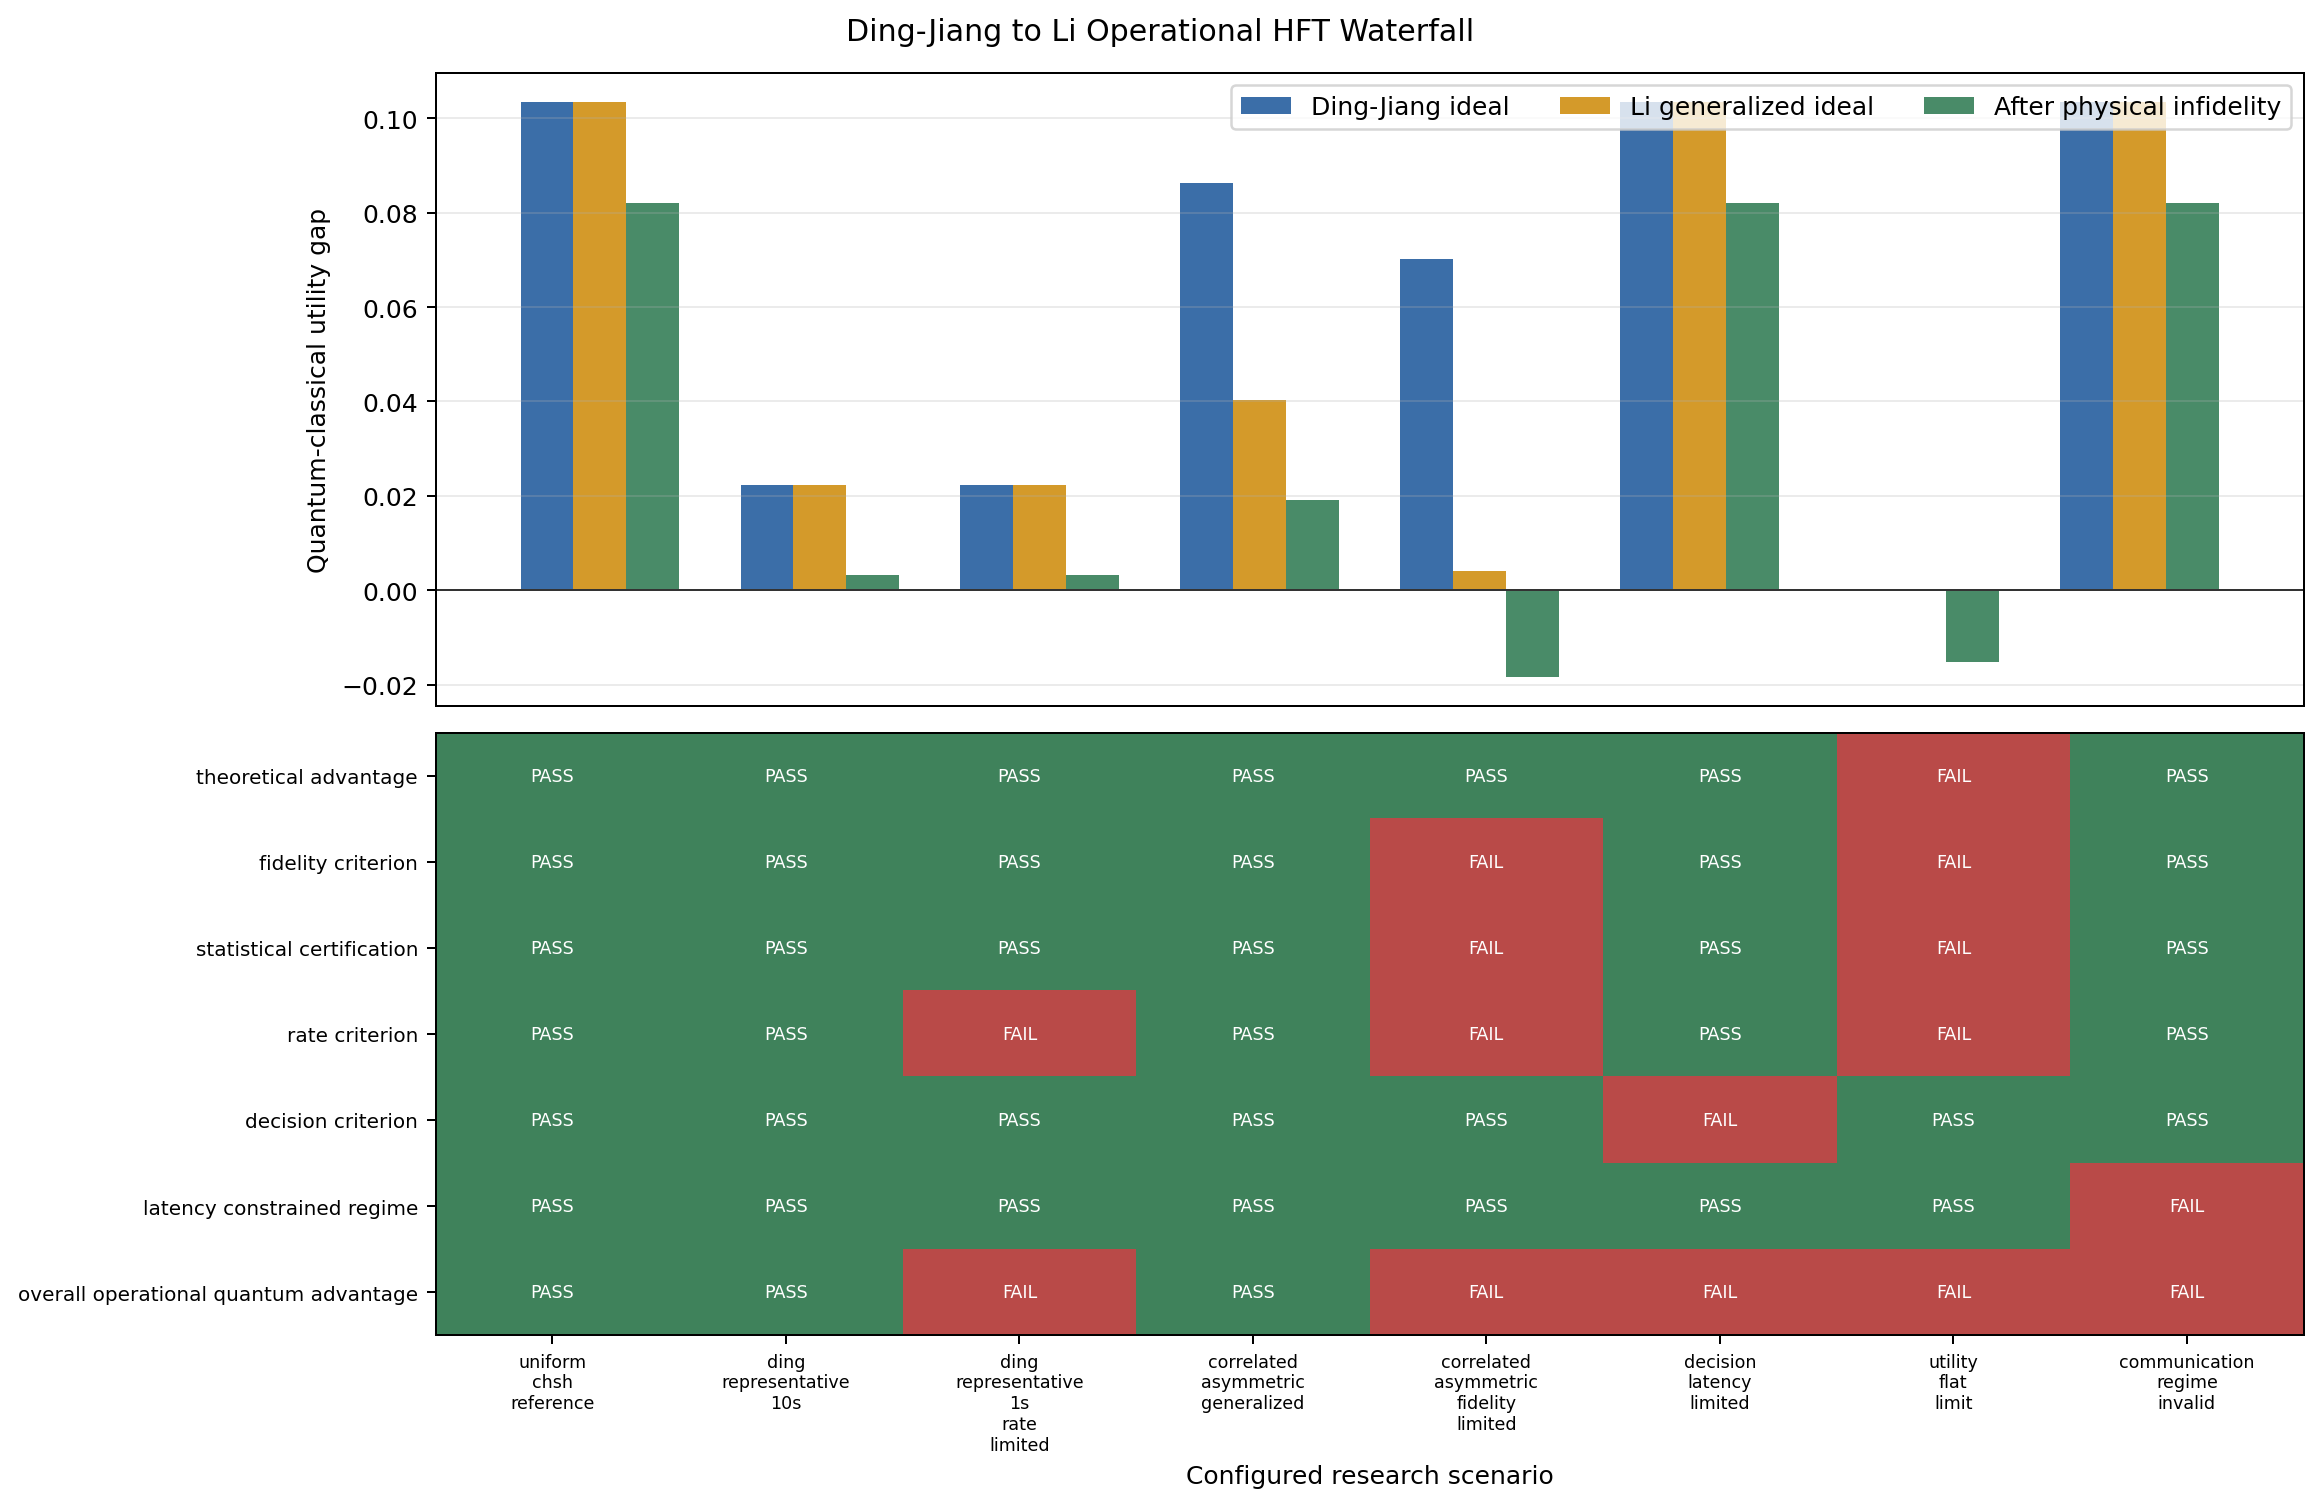
\includegraphics[width=0.93\linewidth]{hft_waterfall.png}
  \caption{Ideal-to-operational HFT decomposition.  Green cells pass the
  corresponding condition and red cells identify the first operational
  obstruction.}
  \label{fig:waterfall}
\end{figure}

The Ding representative case $p=0.3$, $\beta=0.3$ has a noisy gap of only
$0.0032953606$ and requires 66,133 rounds under the bounded-score
certification.  At $T_{\mathrm{env}}=10\,\mathrm{s}$,
$R_{\mathrm{req}}=6613.3\,\mathrm{s}^{-1}$ and the 50-km hardware passes.  At
$T_{\mathrm{env}}=1\,\mathrm{s}$, the same theoretical game requires
$66{,}133\,\mathrm{s}^{-1}$ and fails the rate criterion.  Other controlled
scenarios separately expose fidelity, decision-latency, flat-utility, and
invalid communication-regime failures.  These are sensitivity studies, not
claims based on empirically calibrated market data.

\section{Multiparty Extension and Hardware Search}

The three-party majority-parity game uses all 64 deterministic local
strategies and a GHZ phase strategy.  A second unrestricted three-phase
optimization verifies the symmetric stationary-polynomial production path.
The 101-by-101 grid in Figure \ref{fig:threeparty} reaches the CHSH-sized gap
$0.10355339059327373$ and has 3,474 points above the display positivity
threshold.

\begin{figure}[htbp]
  \centering
  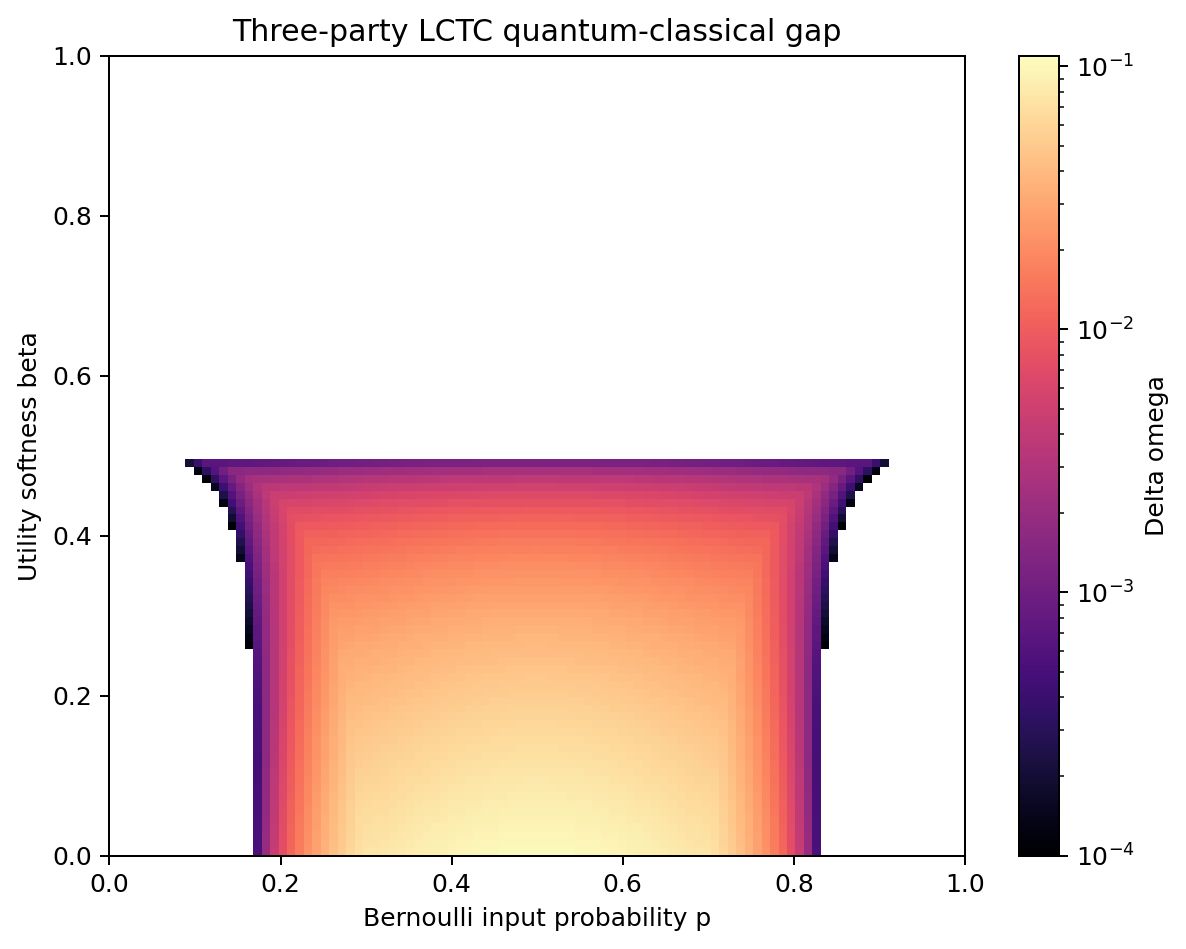
\includegraphics[width=0.70\linewidth]{li_fig7b.png}
  \caption{Equation-level reproduction of Li \emph{et al.} Figure 7(b) for
  the three-party GHZ/XOR extension.}
  \label{fig:threeparty}
\end{figure}

A representative sensitivity case with GHZ state infidelity 0.05 and
measurement infidelity 0.01 has combined infidelity 0.1125904, noisy gap
0.0637467, and $n_{\mathrm{req}}=107$.  It passes when supplied with a 1-MHz
GHZ rate.  The 1-MHz value is a system-level input, not a reproduction of the
microscopic cavity-assisted photon-scattering rate.

Hardware optimization exhaustively evaluates 4,864 finite-grid candidates in
each of nine cases, for 43,776 candidates total.  The objective is simultaneous
satisfaction of theoretical, fidelity, rate, decision, no-communication, and
memory constraints.  An independent dominance scan validates the Pareto set.
Figure \ref{fig:optimization} shows the minimum normalized improvement and the
configured distance envelope.

\begin{figure}[htbp]
  \centering
  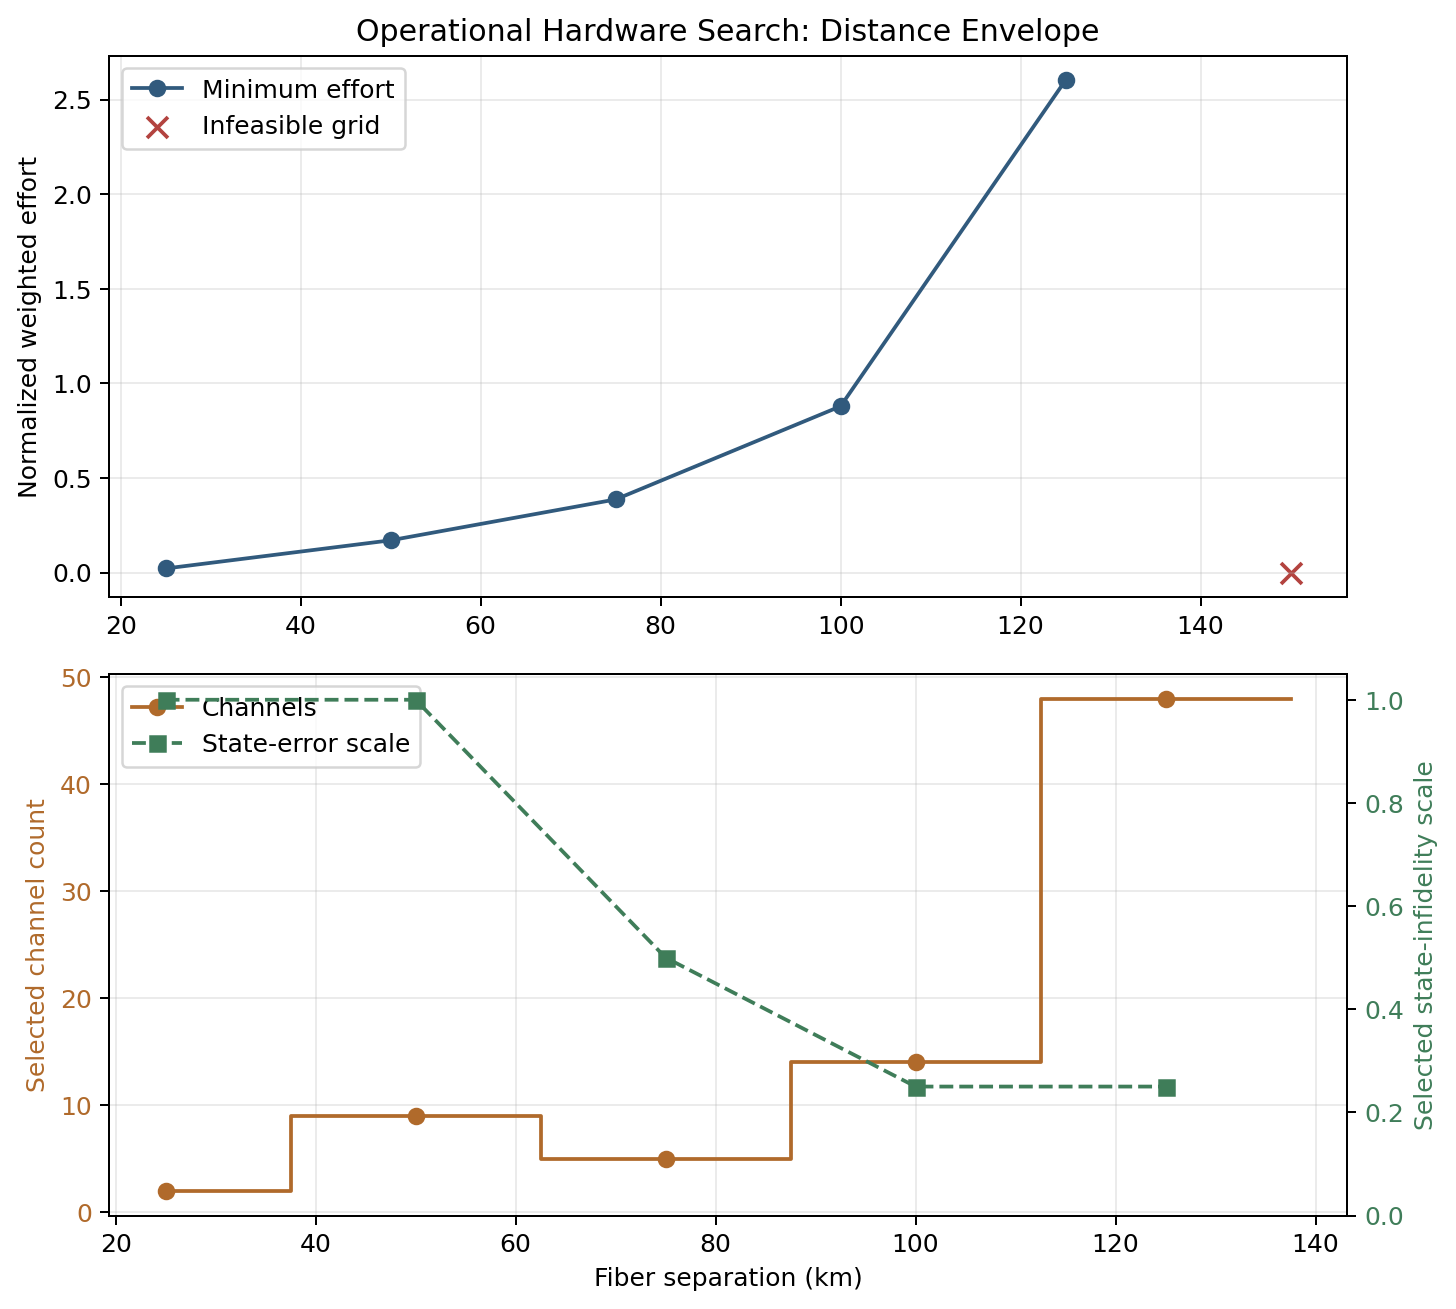
\includegraphics[width=0.90\linewidth]{hardware_optimization.png}
  \caption{Finite-grid hardware-resource optimization.  Normalized effort is
  measured from the Table III baseline to each configured search boundary; it
  is not a monetary or engineering cost.}
  \label{fig:optimization}
\end{figure}

For the Ding 1-s rate-stress case, the 50-km transition requires at least nine
baseline-quality parallel channels.  The configured search finds feasible
designs through 125 km and none at 150 km.  The result is exact only on the
declared finite grid and makes no continuous global-optimality claim.

\section{Final Validation and Scientific Boundaries}

The Phase 15 runner regenerates 12 selected experiment summaries in temporary
directories and compares every scientific value with committed oracles at an
absolute tolerance of $10^{-7}$.  Runtime and generation metadata are excluded.
It also audits JSON configurations, paper-version fields, reproduction-matrix
vocabulary, Git cleanliness of committed results, and result-artifact hashes.
All 12 jobs pass, as do the 592 pre-existing tests and three tests of the Phase
15 artifact itself.  The 45 committed scientific artifacts have aggregate
SHA-256 digest
\begin{center}
\small\texttt{efcdb1d91de1a757007203c0234cdefa1b3d4568996c39bc206486f4ccc84e9a}.
\end{center}

The reproduction matrix contains 35 \pass, 17 \partialstatus, one
\textsc{not implemented}, and three
\textsc{insufficient information} rows.  A computation-level \pass does not
upgrade a paper-level limitation.  The main residual boundaries are:
\begin{itemize}
  \item author pointwise data are unavailable for the reproduced heatmaps;
  \item the Ding Figure 5 full 101-by-101 explicit-strategy surface and
        unpublished modified-NPA code are unavailable;
  \item microscopic two-photon-interference, measurement, and CAPS pulse data
        are insufficient for a faithful device-level reproduction;
  \item the generic nonbinary Bell-operator optimizer is not implemented;
  \item market distributions and utilities are scenario inputs rather than
        empirical market calibration; and
  \item the event model omits jitter and correlated faults.
\end{itemize}

\section{Conclusion}

The simulator independently reproduces the implemented Ding--Jiang ideal HFT
results and connects them, without silently changing their regressions, to the
Li generalized LCTC and operational framework.  The representative 50-km
system illustrates a regime where fidelity, finite statistics, entanglement
supply, and local decision latency can all pass.  The Ding representative HFT
case shows the opposite lesson: a small positive theoretical gap becomes rate
limited when the environment stationary window contracts from 10 s to 1 s.

Operational feasibility is therefore not a property of the nonlocal game
alone.  It is a joint property of utility asymmetry, input correlation, error,
stationarity, hardware throughput, memory occupancy, and local latency.  The
versioned configurations, independent oracles, explicit discrepancies, and
immutable final-validation artifacts make these conclusions reproducible and
falsifiable.  The next scientific priorities are author-data pointwise checks,
microscopic device models once sufficient data are available, correlated-fault
event simulation, empirical market calibration, and continuous multiobjective
resource optimization.

\bibliographystyle{plain}
\bibliography{references}

\end{document}
